% Author: Izaak Neutelings (September 2020)
% Inspiration: https://tex.stackexchange.com/questions/25531/adding-underbrace-in-tikz
\documentclass[border=3pt,tikz]{standalone}
\usepackage{physics}
\usepackage{ifthen}
\usepackage{tikz}
\usetikzlibrary{calc} % for pic
\usetikzlibrary{arrows.meta}
\usetikzlibrary{patterns,snakes}
\usetikzlibrary{angles,quotes} % for pic
\usetikzlibrary{decorations.markings,arrows.meta}
\tikzset{>=latex} % for LaTeX arrow head

\colorlet{myred}{red!65!black}
\colorlet{mydarkblue}{blue!30!black}
\colorlet{xcol}{blue!70!black}
\colorlet{vcol}{green!70!black}
\colorlet{acol}{red!50!blue!80!black!80}
\tikzstyle{vector}=[->,very thick,xcol,line cap=round]
\tikzstyle{force}=[->,myred,thick,line cap=round]
\tikzstyle{Fproj}=[force,myred!40]
\tikzstyle{mydashed}=[dash pattern=on 2pt off 2pt]
\newcommand{\vbF}{\vb{F}}
\def\tick#1#2{\draw[thick] (#1) ++ (#2:0.1) --++ (#2-180:0.2)} %0.03*\xmax
\tikzset{
  midarr/.style={decoration={markings,mark=at position #1 with {\arrow{stealth}}},postaction={decorate}},
  midarr/.default=0.5
}


\begin{document}


% CURVED PATH
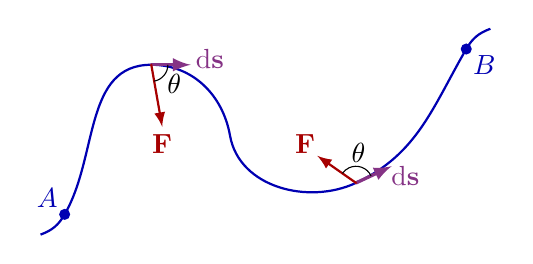
\begin{tikzpicture}
  \def\ul{0.6}
  \def\Ra{1.4}
  \def\Rb{0.8}
  \def\anga{0}
  \def\angb{25}
  \coordinate (A) at (0,0);
  \coordinate (B) at (1.1,1.9);
  \coordinate (C) at (2.1,1.0);
  \coordinate (D) at (3.7,0.4);
  \coordinate (E) at (5.1,2.1);
  
  \draw[xcol,thick]
    (A)++(-140:0.4) to[out=20,in=-120]
    (A) to[out=60,in=\anga-180]
    (B) to[out=\anga,in=100]
    (C) to[out=-80,in=\angb-180]
    (D) to[out=\angb,in=-120]
    (E) to[out=60,in=-160]++ (40:0.4);
  
  % PATH DIFFERENCE
  \draw[vector,acol]
    (B) --++ (\anga:0.5) coordinate (BS) node[above=2,right=-2] {$\dd\vb{s}$};
  \draw[vector,acol]
    (D) --++ (\angb:0.5) coordinate (DS) node[below right=-4] {$\dd\vb{s}$}; %above left=-4
  
  % FORCE
  \draw[force]
    (B) --++ (-80:0.8) coordinate (BF) node[below=-1] {$\vb{F}$};
  \draw[force]
    (D) --++ (145:0.6) coordinate (DF) node[above left=-3] {$\vb{F}$};
  \draw pic["$\theta$",draw=black,angle radius=6,angle eccentricity=1.8] {angle=BF--B--BS};
  \draw pic["$\theta$",draw=black,angle radius=6,angle eccentricity=1.8] {angle=DS--D--DF};
  
  \fill[xcol] (A) circle (2pt) node[above left=-1] {$A$};
  %\fill[xcol] (B) circle (2pt);
  %\fill[xcol] (C) circle (2pt);
  %\fill[xcol] (D) circle (2pt);
  \fill[xcol] (E) circle (2pt) node[below right=-1] {$B$};
  
\end{tikzpicture}


% CLOSED PATH
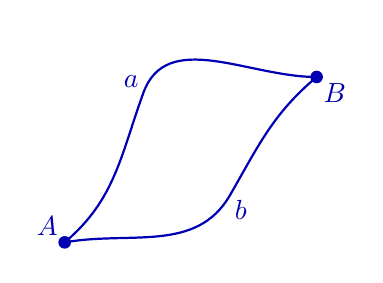
\begin{tikzpicture}
  \def\ul{0.6}
  \def\Ra{1.4}
  \def\Rb{0.8}
  \coordinate (A)  at (0,0);
  \coordinate (Ma) at (1.0,1.9);
  \coordinate (Mb) at (2.1,0.6);
  \coordinate (B)  at (3.2,2.1);
  
  % PATHS
  \draw[xcol,thick]
    (A) to[out=40,in=-110] (Ma) node[above left=-2] {$a$}
        to[out=70,in=-180] (B);
  \draw[xcol,thick]
    (A) to[out=10,in=-120] (Mb) node[below right=-2] {$b$}
        to[out=60,in=-140] (B);
  
  \fill[xcol] (A)  circle (0.08) node[above left=-1] {$A$};
  %\fill[xcol] (Ma) circle (0.08);
  %\fill[xcol] (Mb) circle (0.08);
  \fill[xcol] (B)  circle (0.08) node[below right=-1] {$B$};
  
\end{tikzpicture}


% CONSERVATIVE
\def\xmax{3}
\def\ymax{2.2}
\begin{tikzpicture}
  \def\xa{.21*\xmax}
  \def\xb{.79*\xmax}
  \def\Fa{.22*\ymax}
  \def\Fb{.78*\ymax}
  \def\N{5}
  
  % AREA
  \coordinate (A) at (\xa,\Fa);
  \coordinate (B) at (\xb,\Fa);
  \coordinate (C) at (\xb,\Fb);
  \coordinate (D) at (\xa,\Fb);
  
  % LINE
  \draw[xcol,thick,midarr=0.38] (A) -- (B) node[midway,scale=0.9,left=7,below]     {$a$};
  \draw[xcol,thick,midarr=0.48] (B) -- (C) node[midway,scale=0.9,above=4,right=-1] {$b$};
  \draw[xcol,thick,midarr=0.38] (C) -- (D) node[midway,scale=0.9,right=7,above]    {$c$};
  \draw[xcol,thick,midarr=0.48] (D) -- (A) node[midway,scale=0.9,below=4,left=-1]  {$d$};
  \fill[xcol!70!black] (A) circle (0.04); %node[right=5,above=2] {$P_1$, $V_1$};
  \fill[xcol!70!black] (B) circle (0.04); %node[right=2] {$P_2$, $V_2$};
  \fill[xcol!70!black] (C) circle (0.04); %node[right=2] {$P_2$, $V_2$};
  \fill[xcol!70!black] (D) circle (0.04); %node[right=2] {$P_2$, $V_2$};
  
  % AXIS
  \draw[->,thick] (0,-0.1*\ymax) -- (0,\ymax) node[left] {$y$};
  \draw[->,thick] (-0.1*\xmax,0) -- (\xmax,0) node[below] {$x$};
  \tick{\xa,0}{90} node[below=-1] {$x_1$};
  \tick{\xb,0}{90} node[below=-1] {$x_2$};
  \tick{0,\Fa}{0} node[left=-2] {$y_1$};
  \tick{0,\Fb}{0} node[left=-2] {$y_2$};
  %\draw[<->] (\xa,1.15*\F) -- (\xb,0) node[midway,above=-3,fill=white,inner sep=0] {$\Delta x$};
  
  % FORCE FIELD
  \foreach \i [evaluate={\x=(\i-0.5)*\xmax/\N}] in {1,...,\N}{
    \draw[force] (\x,0.9*\ymax) --++ (0,-0.85*\ymax);
  }
  \node[right=-8,myred] at (1.04*\xmax,0.24*\ymax) {$\vbF = -mg\vu{y}$};
  
\end{tikzpicture}


% CONSERVATIVE - F = (y,x^2)
%http://user.mendelu.cz/marik/EquationExplorer/vectorfield.html
\def\xmax{2.6}
\begin{tikzpicture}
  \def\xa{.21*\xmax}
  \def\xb{.79*\xmax}
  \def\Fa{.22*\ymax}
  \def\Fb{.78*\ymax}
  \def\Nx{4}
  \def\Ny{4}
  \def\wx{\xmax/(\Nx+1)}
  \def\wy{\ymax/(\Ny+1)}
  
  % AXIS
  \draw[->,thick] (0,-0.1*\ymax) -- (0,\ymax) node[left] {$y$};
  \draw[->,thick] (-0.1*\xmax,0) -- (\xmax,0) node[below] {$x$};
  \foreach \i [evaluate={\x=\i*\wx;}] in {1,...,\Nx}{
    \tick{\x,0}{90} node[scale=0.9,below] {\i};
  }
  \foreach \i [evaluate={\y=\i*\wy;}] in {1,...,\Ny}{
    \tick{0,\y}{ 0} node[scale=0.9,left=-1] {\i};
  }
  
  % AREA
  \coordinate (A) at (0,0);
  \coordinate (B) at ({2*\wx},{4*\wy});
  \node[right=1,below left=-1] at (A) {$(0,0)=A$};
  \node[right] at (B) {$B = (2,4)$};
  \node[right,myred] at (0.5*\xmax,0.4*\ymax) {$\vbF = y\vu{x} + x^2\vu{y}$};
  
  % LINE
  \draw[xcol,thick,midarr=0.6] (A) -- (B) node[midway,scale=0.9,above left=-1] {$a$};
  \draw[xcol,thick,variable=\x,samples=100,smooth,domain={0:2}] %,midarr=0.6
    plot({\wx*\x},{\wy*\x*\x});
  \draw[-stealth,xcol] ({\wx*1.3},{\wy*1.3^2}) --++ (65:0.01) node[below right=-2] {$b$}; %-{stealth[length=8,width=8]}
  \fill[xcol!70!black] (A) circle (0.04); %node[right=5,above=2] {$P_1$, $V_1$};
  \fill[xcol!70!black] (B) circle (0.04); %node[right=2] {$P_2$, $V_2$};
  
\end{tikzpicture}


\end{document}